\documentclass[12pt]{beamer}
\usepackage{tikz}
\usepackage[italian]{babel}
\usepackage{minted}

\usetheme{Madrid}
\usecolortheme{orchid}

\definecolor{blue}{HTML}{608bf6}
\definecolor{black}{HTML}{1c1c1c}
\definecolor{green}{HTML}{39e600}
\definecolor{grey}{HTML}{949494}

\title{Introduzione alle CTF}
\subtitle{Lezione 1}
\author{Alessandro Righi \and Cristiano Di Bari}
\institute{Università degli Studi di Verona}
\date{9 Novembre 2023}

\begin{document}
\begin{frame}
\titlepage
\end{frame}

\section{Introduzione}

\begin{frame}{Chi siamo?}
\begin{columns}[T] % align columns
\begin{column}{.48\textwidth}
\begin{itemize}
\item laurea magistrale @ UniVR
\item istruttore @ CyberChallenge
\item \textit{System Developer} @ IOTINGA
\end{itemize}        
{\color{blue}\rule{\linewidth}{2pt}}%
\begin{center}
Cristiano Di Bari
\begin{tikzpicture}[inner ysep=0.4cm]
\clip (0,0) circle (1.5cm) node {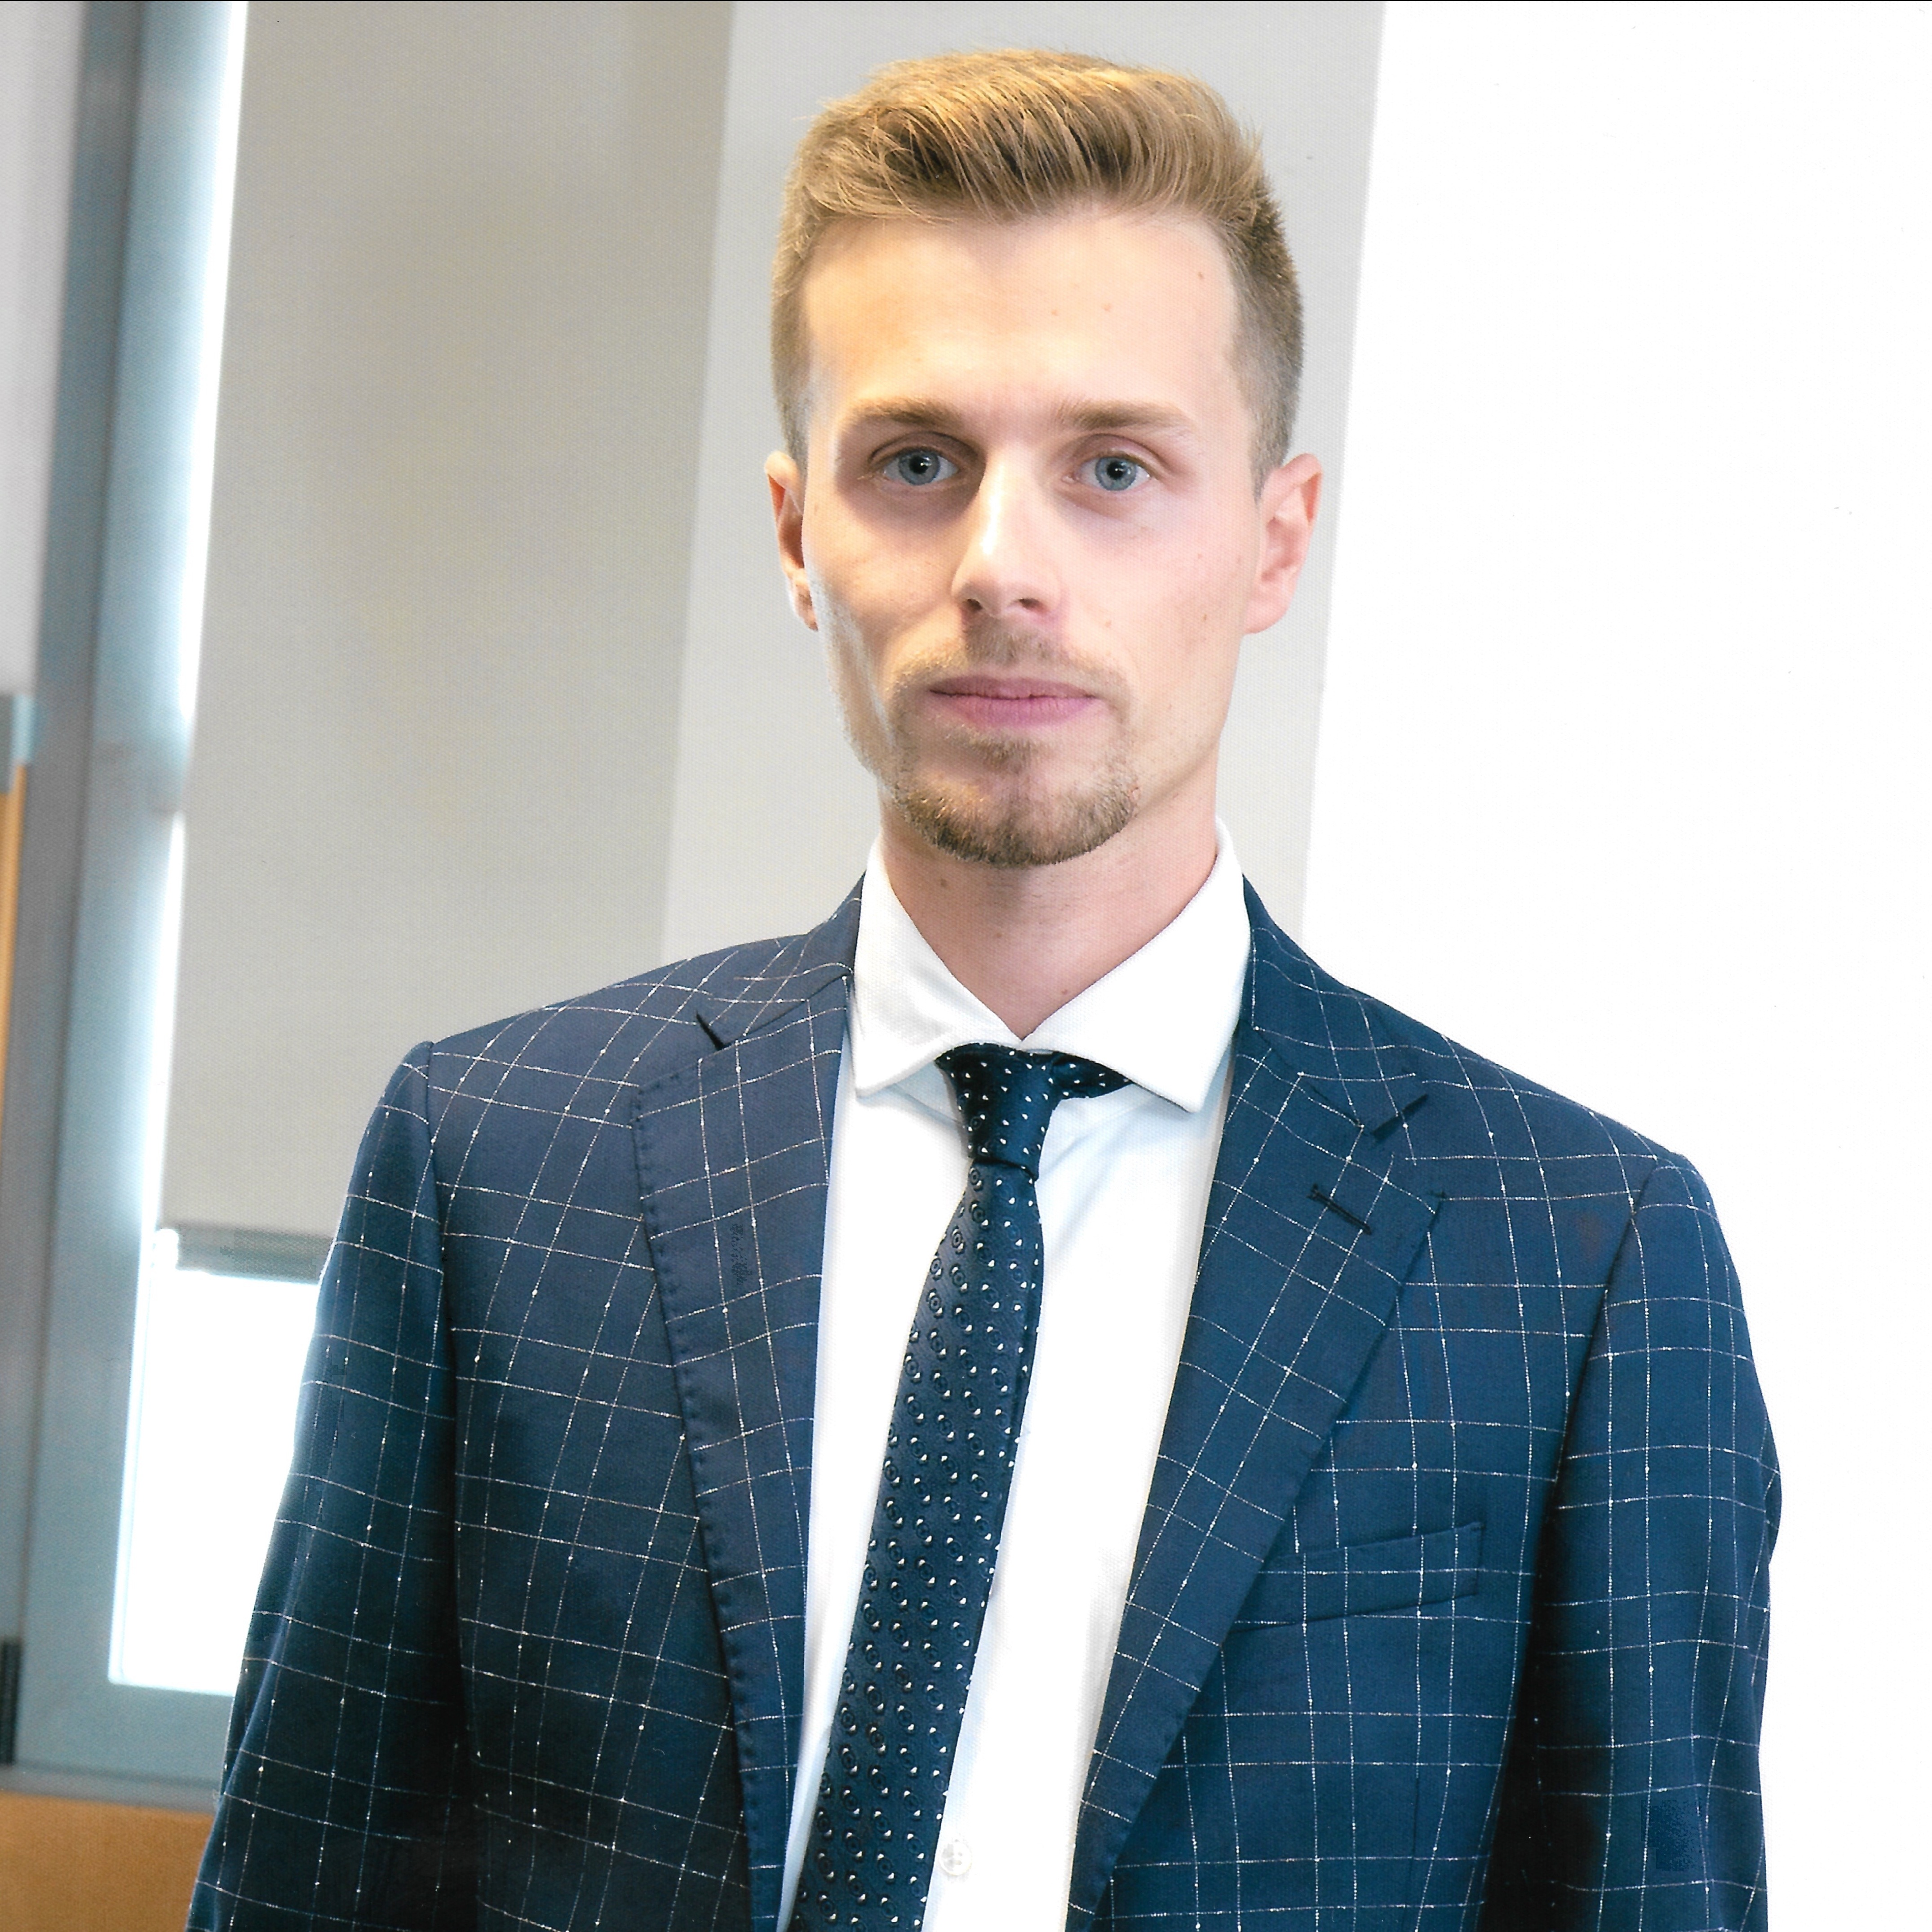
\includegraphics[width=3cm]{img/cris.jpg}};
\end{tikzpicture}
\end{center}
\end{column}%
\hfill%
\begin{column}{.48\textwidth}%
\begin{center}%
\begin{tikzpicture}%
\clip (0,0) circle (1.5cm) node {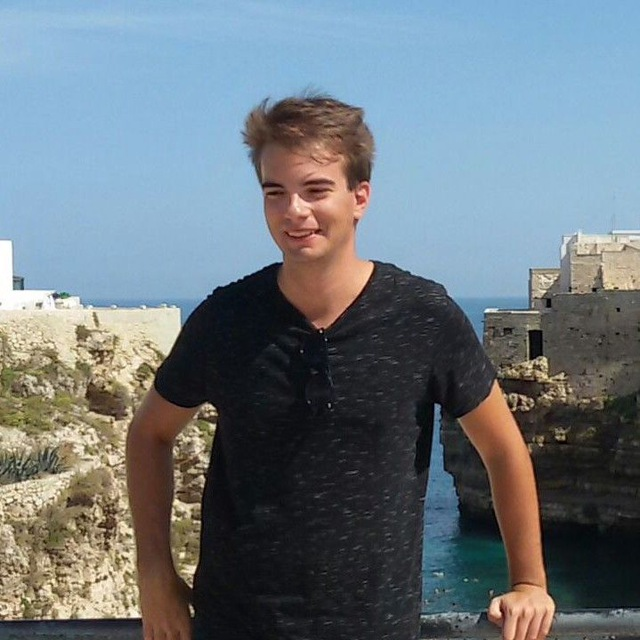
\includegraphics[width=3cm]{img/ale.jpeg}};
\end{tikzpicture}

Alessandro Righi
\color{blue}{\rule{\linewidth}{2pt}}%
\begin{itemize}
\item laurea magistrale @ UniVR
\item istruttore @ CyberChallenge
\item \textit{Applied Research Director} @ IOTINGA
\end{itemize}
\end{center}
\end{column}%
\end{columns}
\end{frame}

\begin{frame}{Cosa sono le CTF?}

Le \textit{Capture The Flag} (CTF) sono delle sfide in cui i partecipanti 
devono trovare delle \textit{flag}, ossia delle stringhe di testo, all'interno
di sistemi informatici contenenti delle vulnerabilità di sicurezza. 
\vfill
\begin{exampleblock}{Esempio di flag}
\texttt{CCIT\{Th1s-1sY0uR-F1rst-Fl4ag\}}
\end{exampleblock}
\vfill
Una volta trovate le flag vanno, solitamente, inviate ad una piattaforma di gara, 
che si occupa di validarle, assegnando il punteggio della challenge nel caso siano corrette.
\end{frame}

\begin{frame}{Perché fare CTF?}
Avete mai fatto CTF?

\pause\vfill

Se no... ecco alcune ragioni per iniziare:
\pause\vfill
\begin{itemize}
\item per divertirsi!
\pause\vfill
\item per imparare cose nuove (tante)
\pause\vfill
\item per scrivere software (più) sicuro
\pause\vfill
\item per conoscere nuova gente, creare networking
\end{itemize}
\end{frame}

\begin{frame}{Tipologie di CTF}
Esistono due tipologie di CTF:
\begin{itemize}
    \item \textit{Jeopardy}: il partecipante attacca una serie di servizi malevoli e sottomette le flag ad un sistema di verifica
    \item \textit{Attack-Defence (AD)}: competizione a squadre dove ogni team deve attaccare i sistemi dell'avversario, e difendere i propri
\end{itemize}

\vfill
Per queste lezioni di concentreremo sul primo tipo (\textit{Jeopardy}), di gran lunga le più diffuse, che è anche
quella organizzata da \textit{Würth Phoenix}.
\end{frame}

\begin{frame}{Tipologie di challenge}
Tipicamente le challenge che si affrontano possono essere di 4 macro categorie:
\begin{itemize}
    \item \textit{Binary}: è necessario ricercare vulnerabilità in un eseguibile, quali ad es. buffer overflow
    \item \textit{Web}: si tratta di trovare vulnerabilità in una web app, web API, o comunque applicativo esposto in rete
    \item \textit{Crypto}: è necessario decodificare un testo cifrato con un algoritmo (ovviamente vulnerabile)
    \item \textit{Misc}: sono challenge che non rientrano in nessuno dei tipi precedenti, e richiedono spesso creatività per essere affrontate
\end{itemize}

Per queste lezioni ci concentreremo sulla categoria \textit{Web}.
\end{frame}

\begin{frame}
\Huge\center Iniziamo!
\end{frame}

\section{Path traversal}
\subsection{Introduzione}
\begin{frame}{Path traversal}

Immaginiamo di avere una pagina web che per caricare l'immagine del profilo di un utente effettua una richiesta a:

\begin{exampleblock}{Richiesta}
\texttt{https://mysecureapp.com/assets?name=image.jpeg}
\end{exampleblock}

\pause
\vfill
Cosa succede se modifico la richiesta in questo modo?

\begin{exampleblock}{Richiesta alterata}
\texttt{https://mysecureapp.com/assets?name=../index.php}
\end{exampleblock}
    
\pause

Se il server non effettua adeguati controlli, è possibile leggere file fuori dalla \textit{root} directory del web server!

\end{frame}
\begin{frame}{Path traversal}
Cosa consente di fare questa vulnerabilità?
\vfill
\pause
\begin{itemize}
    \item leggere \textit{segreti} altrimenti non accessibili, ad es. file di configurazione quali \texttt{/etc/passwd}
    \pause
    \item ottenere il \textit{codice sorgente} dell'applicazione web
    \pause
    \item accedere ai dati di altri utenti, bypassando restrizioni imposte dall'applicazione web
    \pause
\end{itemize}

\vfill
\begin{block}{Suggerimento}
È possibile aggiungere tanti \texttt{../} fino a raggiungere la directory \textit{root}, ad esempio \texttt{../../../../../etc/passwd}
\end{block}

\end{frame}
\subsection{Challenges}
\begin{frame}{Challenges}
Vediamo la prima challenge. Per queste lezioni utilizzeremo delle challenge 
prese dalla piattaforma di allenamento delle Olimpiadi di Cybersecurity (\url{https://olicyber.it}), 
a cui vi invitiamo ad iscrivevi.
\end{frame}

\begin{frame}{Traverse me}
    \url{https://training.olicyber.it/challenges\#challenge-504}
    \vfill
    Ho trovato questa galleria di quadri, chissà se ce ne sono di nascosti.
    \vfill
    \pause
    \begin{itemize}
        \item In questa applicazione vengono caricati dei file salvati sul server, sai individuare dove?
        \pause
        \item Forse è possibile modificare il nome del file per visualizzare altri elementi presenti sul filesystem.
        \pause
    \end{itemize}
    \vfill
    \begin{exampleblock}{Domanda}
        É possibile stampare altri file?
    \end{exampleblock}
\end{frame}

\begin{frame}{Traverse me more}
    \url{https://training.olicyber.it/challenges\#challenge-507}
    \vfill
    Questa volta ho fixato il problema della galleria d'arte, non riuscirai mai a carpire il mio segreto.
    \vfill
    \pause
    \begin{itemize}
        \item Provando ad applicare la soluzione per la challenge precedente ci accorgiamo che non funziona!
        \pause
        \item Guardando il codice sorgente, notiamo che viene fatto un \textit{sanitize} del nome del file che rimuove alcuni caratteri.
        \pause
        \item Possiamo bypassare questo controllo?
        \pause
    \end{itemize}
\end{frame}

\begin{frame}{Light or dark}
    \url{https://training.olicyber.it/challenges\#challenge-49}
    \begin{itemize}
        \item La challenge mostra un sito web in cui è possibile selezionare il tema, come viene applicato lo stile alla pagina html?
        \pause
        \item Scaricando il file sorgente php notiamo che lo sviluppatore ha applicato dei filtri per evitare che un utente malintenzionato possa caricare un file diverso dai fogli css.
        \pause
        \item Il secondo controllo verifica che l'estensione del file da caricare sia \texttt{.css}, in caso contrario aggiunge l'estensione richiesta tramite una concatenazione di stringhe. Questo controllo sembra difficile da aggirare...o forse no.
        \pause
    \end{itemize}

    \begin{block}{Suggerimento}
        Avete mai sentito parlare di ``Null Byte Injection''?
    \end{block}
\end{frame}


% \subsection{Tool: Burp suite}
\begin{frame}{Burp Suite}
    Introduciamo un tool che ci sarà utile per le prossime challenge. 
    \vfill
\begin{itemize}
    \item Il tool \textit{Burp Suite} (scaricabile in versione community gratuitamente) agisce 
        come proxy HTTP
    \item Agendo da proxy blocca le richieste HTTP fra il browser ed il server, e consente di ispezionarle, eventualmetne modificarle e quindi farne il forward al server.
    \item Include anche una serie di utilità, ad esempio la possibilità di decodificare valori in vari formati, ad esempio base64.
\end{itemize}
    \vfill
    Vediamone una demo!
\end{frame}

\begin{frame}{Flags shop}
    % https://training.olicyber.it/challenges#challenge-43
    \begin{itemize}
        \item La challenge mostra un sito web dal quale è possibile acquistare dei prodotti
        \pause
        \item Forse guardare le richieste che effettua l'applicazione web aiuta?
        \pause
        \item Il parametro prezzo sembra un po' sospetto... 
    \end{itemize}

    \begin{exampleblock}{Domanda}
        Quale tool visto prima potrebbe agevolarci nello svolgimento di questa challenge?
    \end{exampleblock}
\end{frame}

%%% SQLI 

\section{SQL Injection}
\begin{frame}[fragile]{SQL Injection}
\begin{minted}{PHP}
<?php
$user = mysql_query("SELECT * FROM users WHERE 
    username = '$username' AND password = '$password');
if (!$user) {
    echo "utente non trovato!";
} else {
    echo "Accesso eseguito!";
}
\end{minted}
\vfill
\begin{exampleblock}{Domanda}
    Il codice in questa slide è sicuro?
\end{exampleblock}
\end{frame}

\begin{frame}{SQL Injection}
    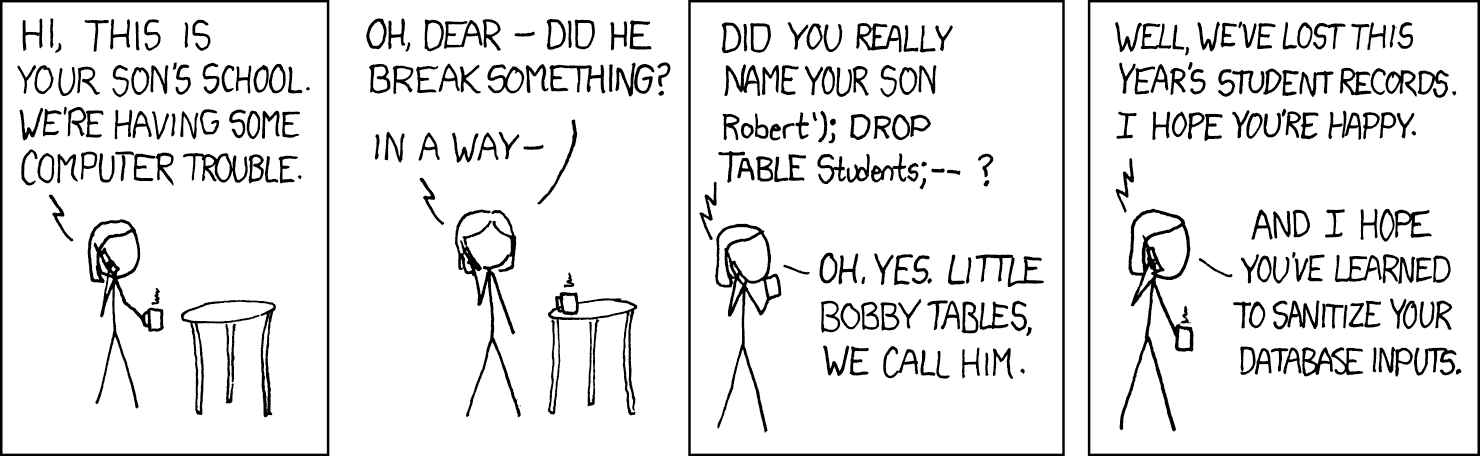
\includegraphics[width=\textwidth]{img/sqli.png}
    \url{https://xkcd.com/327/}
\end{frame}
    
\begin{frame}[fragile]{SQL Injection}
Vediamo cosa accade andando a settare la variabile username al valore \texttt{"admin'--"}:
\vfill
\begin{minted}{SQL}
SELECT * FROM users WHERE 
username = 'admin'--' AND password = 'boh'
\end{minted}
\pause
\vfill
Il controllo della password è completamente stato eluso!
\vfill
\begin{alertblock}{Prevenzione}
Mai compore query SQL interpolando stringhe!
\end{alertblock}

\end{frame}

\begin{frame}{SQL Injection}
\begin{itemize}
\item le SQL injection rientrano nella più ampia categoria delle \textit{code injection}
\item le SQL injetion sono \textit{purtroppo} ancora una delle vulnerabilità più diffuse
\item in questo caso, si trattava di una \textit{blind} SQL injection, in quanto il risultato non è direttamente riflesso all'utente
\item usa sempre i \textit{prepared statement} messi a disposizione della libreria che usi per interrogare il database per effettuare query!
\end{itemize}
\end{frame}

\begin{frame}{Basic SQLi}
\url{https://training.olicyber.it/challenges\#challenge-48}
\vfill
\begin{itemize}
    \item il titolo dice tutto!
    \pause
    \item ricorda la slide precedente... 
    \pause
    \item SQL supporta altri caratteri per aggiungere commenti
\end{itemize}

\end{frame}

\begin{frame}{Admin's secret}
\url{https://training.olicyber.it/challenges\#challenge-44}
\vfill
\begin{itemize}
    \item analizza attentamente il codice sorgente
    \pause
    \item nel login vengono usati i prepared statement, forse il problema è nella registrazione
    \pause
    \item riesci a creare un utente di tipo admin?
\end{itemize}

\end{frame}

\begin{frame}{Password changer 3000}
    \url{https://training.olicyber.it/challenges\#challenge-59}
    \vfill
    Riesci a cambiare la password dell'utente "admin"?
    \begin{itemize}
        \item Un sito per cambiare le password degli utenti...non sembra molto utile.
        \pause
        \item Provando a cambiare la password dell'utente ``pippo'' otteniamo in risposta una nuova password. Proviamo ad analizzare la richiesta HTTP che abbiamo appena effettuato. 
        \pause
        \item Dovremmo riuscire ad impersonare l'utente ``admin'', forse la codifica \texttt{Base64} può esserci d'aiuto.
        \pause
    \end{itemize}
\end{frame}

\begin{frame}{Curl}
\begin{itemize}
    \item per le prossime challenge, sarà necessario effettuare richieste HTTP a servizi REST. 
    \item esistono svariati tool per farlo, quali \textit{Insomnia}, \textit{Postman}, etc.
    \item vediamo brevemente il tool da riga di comando \textit{curl}
    \item molto probabilmente lo hai già installato sul tuo sistema
\end{itemize}
\vfill
\begin{alertblock}{Per gli utenti Windows}
Utilizza il comando \texttt{curl.exe} in quanto \texttt{curl} usa opzioni diverse.
\end{alertblock}
\end{frame}

\begin{frame}{Curl}
\begin{itemize}
    \item GET: \texttt{curl -v http://example.com}
    \item POST: \texttt{curl -v -X POST http://example.com -d "body"}
    \item set di un header: \texttt{curl -v -H 'chiave: valore' http://example.com}
\end{itemize}
\vfill
\begin{block}{Suggerimento}
Dagli strumenti di sviluppo di Firefox e Chrome nella pagina \textit{Rete} è possibile copire il comando curl di una richiesta nel menù che appare cliccando con il tasto destro così da poterlo incollare nel terminale
\end{block}
\end{frame}

\begin{frame}{A TOO small reminder...}
\url{https://training.olicyber.it/challenges\#challenge-36}
\vfill
\begin{itemize}
    \pause
    \item assicurati di specificare il \textit{Content-Type} corretto!
    \pause
    \item non sembrano esserci vulnerabilità nel login
    \pause
    \item guarda attentamente il cookie di sessione che viene assegnato, noti nulla?
    \pause
    \item possiamo presumere che l'admin abbia una sessione aperta
\end{itemize}
\pause
\vfill
\begin{alertblock}{Prevenzione}
I cookie di sessione dovrebbero essere impossibili da indovinare
\end{alertblock}
\end{frame}

\begin{frame}{ZioFrank}
\url{https://training.olicyber.it/challenges\#challenge-53}
\vfill
\pause
\begin{itemize}
    \item la vulnerabilità non è un SQL injection
    \pause
    \item controlla \textit{attentamente} lo schema dei dati
    \pause
    \item sembra che venga effettuata una query separata per capire se l'utente è admin
    \pause
    \item qualcosa previene il creare un nuovo utente con lo stesso username di uno esistente?
    \pause
\end{itemize}
\vfill
\begin{block}{Suggerimento}
È sempre buona norma definire le colonne univoche con \texttt{UNIQUE}
\end{block}

\end{frame}

\begin{frame}[fragile]{Cross-Site Scripting}
\begin{minted}{javascript}
    document.innerHTML = "Benvenuto, " + username
\end{minted}
\vfill
\begin{exampleblock}{Domanda}
Cosa c'è di sbagliato in questo codice apparentemente innocuo?
\end{exampleblock}
\end{frame}

\begin{frame}{Cross-Site Scripting}
\begin{itemize}
\item cosa accade se username contiene degli elementi HTML?
\pause
\item in particolare, se contiene dei tag \texttt{<script>}?
\pause
\item è possibile far eseguire del codice JavaScript a chiunque apra quella pagina!
\pause
\item ad esempio, possiamo leggere il cookie di sessione e farlo inviare ad un nostro server
\pause
\item oppure fare richieste alla pagina stessa con i cookie dell'utente
\end{itemize}
\pause
\vfill
\begin{alertblock}{Prevenzione}
Usa sempre un framework o una libreria che si occupa di sanificare il testo che inserisci nelle pagine HTML dinamiche!
\end{alertblock}
\end{frame}

\begin{frame}{Fine}
Ci auguriamo che queste due lezioni ti abbiano lasciato più che altro curiosità di approfondire gli aspetti di sicurezza!
\vfill
Se sì... hai mai sentito parlare della \textit{CyberChallenge}?
\end{frame}

\end{document}
